\section{Model selection} \label{sec:modelselection}

First, we train the network only on synthetic data generated by starGen, which has a total of 172 800 images. The network has a large number of hyperparameters, which need to be tuned to recognize objects correctly. In this section, we present the process of selecting the best-performing parameters for the network. During training, the network is validated using both synthetic and real images. The validation set contains 96 000 synthetic and 300 real images. After selecting the configuration of parameters that works best on the validation set, we evaluate the model on testing data, which consists of 300 real images.  

\subsection{Baseline model}

After generating the first iteration of data, we used it to train multiple models and test the parameters of the network. Based on the best configuration, we established a baseline model with following parameters:

\begin{itemize}
    \setlength\itemsep{1px}
    \item activation function Leaky RELU with a slope of 0.05 
    \item batch size of 32
    \item optimizer ADAM with betas = 0.9, 0.999
    \item learning rate of $1e^{-3}$ without a scheduler
    \item dropout in fully-connected layer with probability = 0.5
    \item no L2 regularization applied
\end{itemize}

The baseline model is then used on all iterations of data, where we configure the parameters again. This process is documented in the following sections. 
\subsection{Training specifications}
We have talked about hyperparameters of the network that we need to tune, but there are also some specifications of the training, itself. These settings are used during the training on all of the models. 

\subsubsection{Early stopping algorithm}

The training process is observed by the early stopping algorithm, which stops the training after the validation loss is not improving for a certain period. However, after training several models we have noticed that the lowest validation loss for real data doesn't correspond to the highest accuracy. This may be due to some outliers in the validation set that increase the loss, even though the classification performs adequately. 

This phenomenon is shown in the Figure \ref{fig:esalossacc1}, where we show the progress of the validation loss and accuracy during the training of one of the models. You may notice that from a certain epoch the validation loss on the real data (orange line) starts to increase (Figure \ref{fig:loss1}) and the early stopping algorithm stops the training after some time. However, if we look at the progress of the accuracy (Figure \ref{fig:acc1}) we see that at that exact point (red dotted line) the accuracy starts to increase. The model should be trained for more epochs but since the early stopping algorithm stops the training, we can't achieve better accuracy. 

To prevent this problem we have decided to use accuracy instead of loss for the early stopping algorithm. Based on some observations, we have noticed that loss and accuracy on the synthetic validation set follow a similar path as accuracy and loss on the training set. For this reason, we are using accuracy on the real images in the validation set.  

The training will proceed for 100 epochs and stops if the validation accuracy doesn't improve after 10 epochs. This waiting time of 10 epochs is also referred to as a parameter patience. 

\begin{figure}[!h]
\centering
    \begin{subfigure}[t]{.45\textwidth}
        \centering
        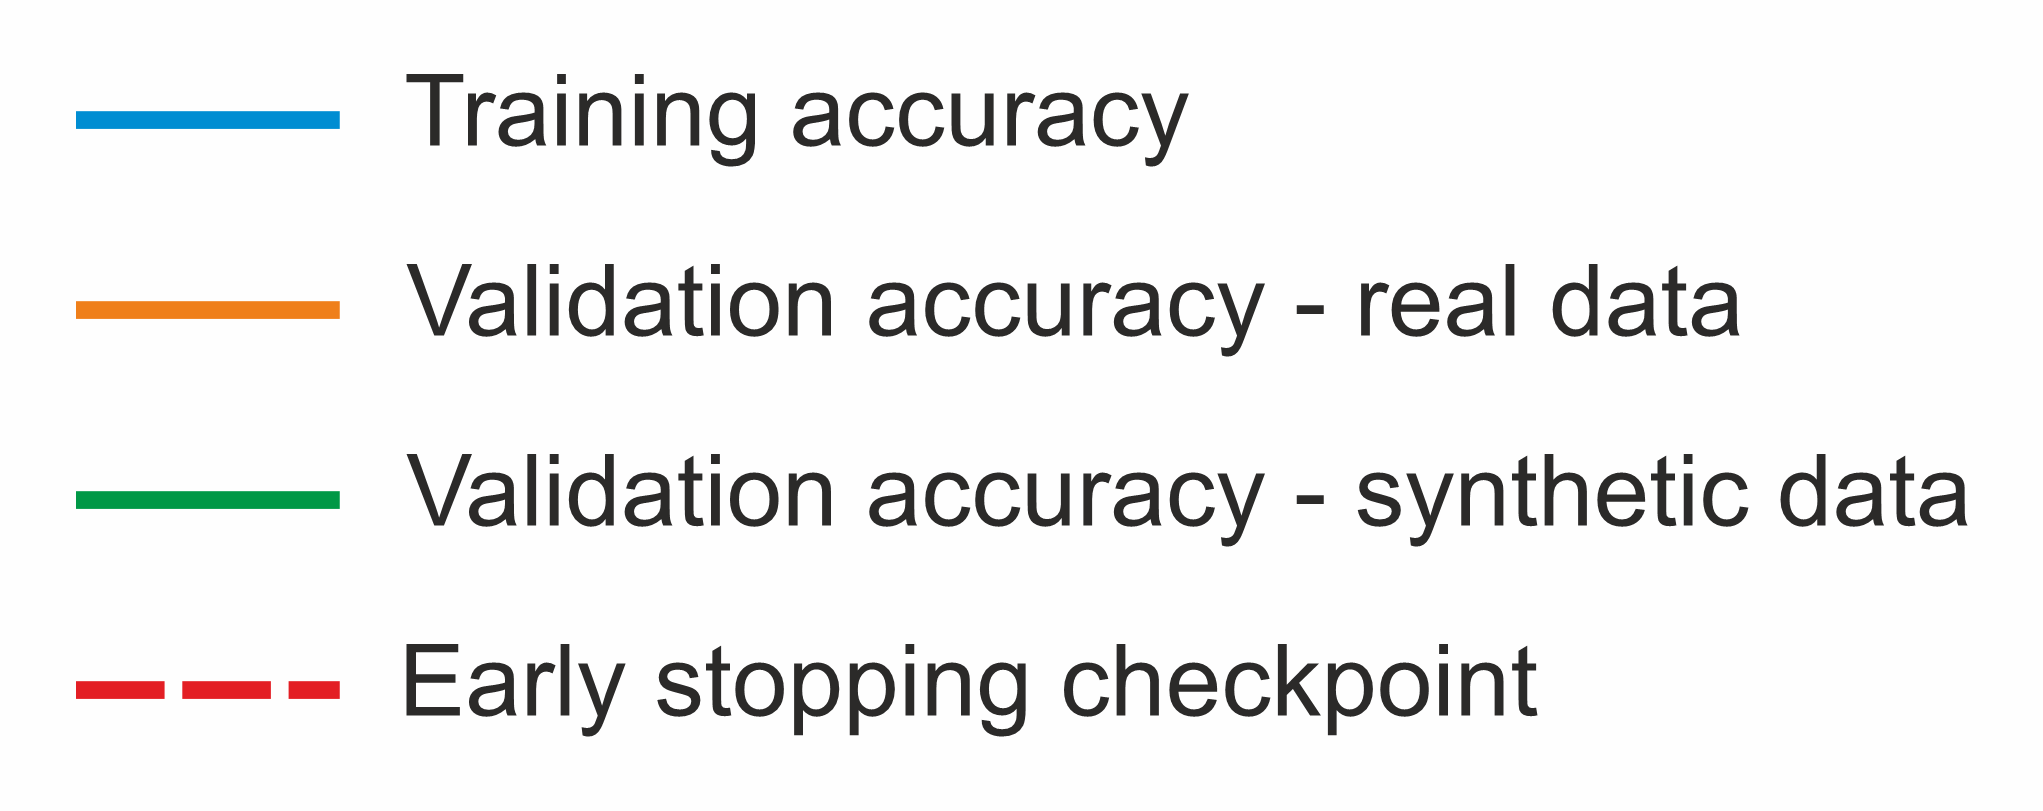
\includegraphics[width=.7\textwidth]{images/popisAc.png}
        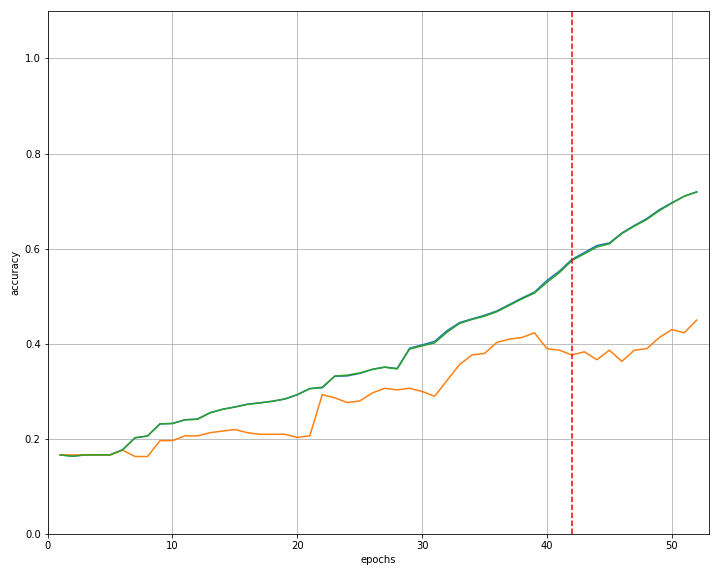
\includegraphics[width=\textwidth]{images/accuracy1ss_0.png}
        \caption{Evolution of the accuracy during training.}
        \label{fig:acc1}
    \end{subfigure}
    \begin{subfigure}[t]{.45\textwidth}
        \centering
        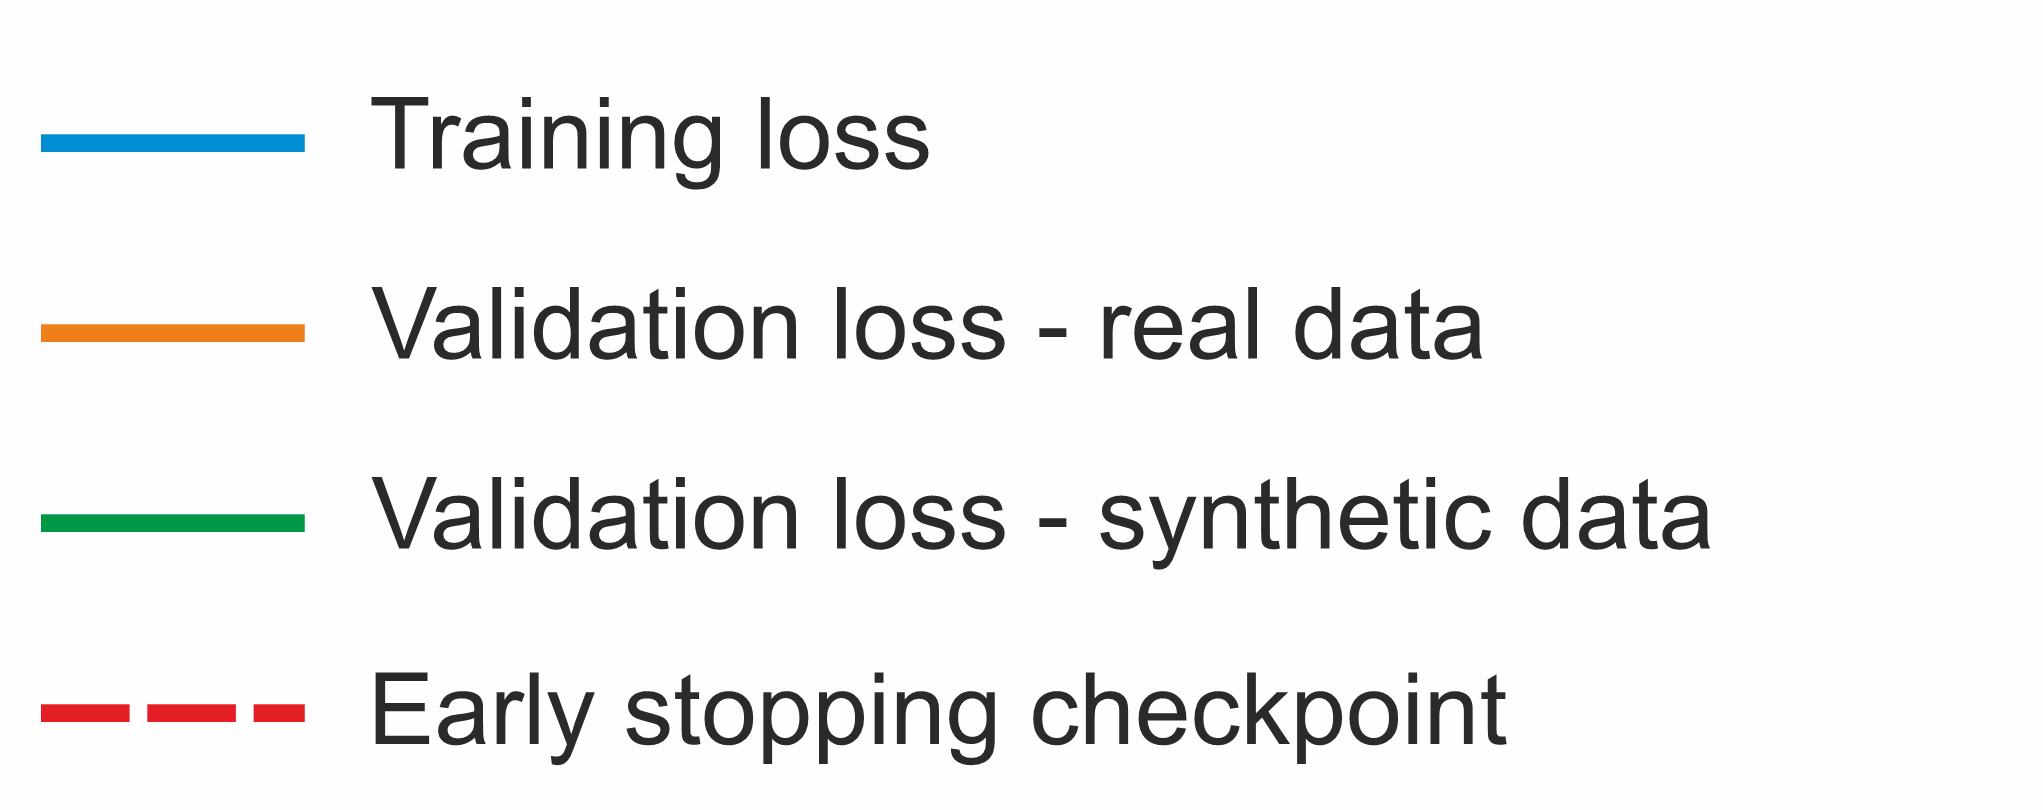
\includegraphics[width=.7\textwidth]{images/popisLoss.png}
        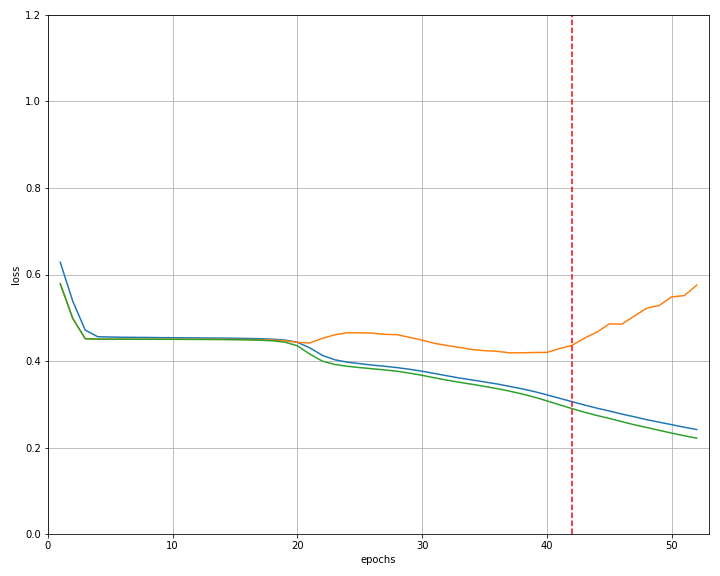
\includegraphics[width=\textwidth]{images/losses1ss_0.png}
        \caption{Evolution of the loss during training.}
        \label{fig:loss1}
    \end{subfigure}

    \caption{The increase of both the accuracy and the loss on the validation set of real images from a checkpoint.}
    \label{fig:esalossacc1}
\end{figure}


\subsubsection{Multiple models}

Training of the network also depends on some random operations like initial values of the weights or the division of images into batches. To avoid the randomness affecting our results, we train 10 models on each configuration of parameters. The provided metrics are then measured as average over all 10 models. 
\subsubsection{Activation function}

Activation function is used for non-linearity in forward pass of the network. Function takes one number and performs defined mathematical operation on it. In our work we will be testing following activation functions:
\begin{itemize}
    \item \textit{Sigmoid activation}
        \begin{equation}
            \sigma (x) = \frac{1}{1 + e^{-x}}
        \end{equation}
        
    \item \textit{Hyperbolic tangent activation (tanh)}
        \begin{equation}
            tanh(x) = \frac{2}{1+e^{-2x}} - 1
        \end{equation}
    
    \item \textit{Rectified Linear Unit (RELU) activation}
        \begin{equation}
            f(x) = max(0,x)
        \end{equation}
        
    \item \textit{Leaky RELU activation}
        \begin{equation}
            f(x) = 
            \begin{cases}
                x,& \text{if } x\geq 0\\
                \alpha x ,& \text{otherwise}
            \end{cases}
        \end{equation}
\end{itemize}

Each activation has its advantages and disadvantages. Sigmoid was a very popular choice in the past as it was the closest approximation to the firing of the neuron in a biological sense. However, large negative and positive numbers get saturated, which results in a gradient close to zero. During backpropagation, this will kill the flow of the gradient and the network won't be able to learn. Another undesirable feature of the sigmoid is that it is not zero-centered which makes the gradient updates follow a zig-zag pattern. On the other hand tanh activation outputs zero-centered values but similar to sigmoid, large values get saturated. Nowadays, the most used activation is RELU activation. Positive numbers don't get saturated as they follow a linear path. Yet large gradient update of weights could cause the input values to RELU neurons to be always negative. This way the neuron always outputs zero, doesn't contribute to the learning process of the network and essentially "dies". One way to fix the problem is introduced by Leaky RELU. Instead of outputting zero when negative inputs come, the function multiplies the negative value with a small constant $\alpha$ \cite{standford}.

\subsection{Batch size}

We mentioned that the images fed to the network come in mini-batches to increase the speed of the training. The size of the batch is determined by the parameter batch size. It is a common practice the use powers of 2 for the size which is why we have decided to do the same. 

Again we chose the baseline model to train and used different sizes of mini-batches. Results on the validation set are shown in the Table \ref{tab:batchsizetab}. 

{\renewcommand{\arraystretch}{1.3}
\begin{table}[h]
\centering
\begin{tabular}{|l|cc|cc|}
\hline
\multicolumn{1}{|c|}{\multirow{2}{*}{\textbf{Batch size}}} & \multicolumn{2}{c|}{\textbf{Validation loss}} & \multicolumn{2}{c|}{\textbf{Validation accuracy (\%)}} \\ \cline{2-5} 
\multicolumn{1}{|c|}{} & \multicolumn{1}{c|}{real data} & synthetic data & \multicolumn{1}{c|}{real data} & synthetic data \\ \hline
\textit{8} & \multicolumn{1}{c|}{4.830184} & 0.005608 & \multicolumn{1}{c|}{76.66} & 99.48 \\ \hline
\textit{16} & \multicolumn{1}{c|}{2.562120} & 0.005470 & \multicolumn{1}{c|}{80.00} & 99.50 \\ \hline
\textit{32} & \multicolumn{1}{c|}{1.017293} & 0.006852 & \multicolumn{1}{c|}{79.33} & 99.31 \\ \hline
\textit{64} & \multicolumn{1}{c|}{0.958888} & 0.005262 & \multicolumn{1}{c|}{80.00} & 99.53 \\ \hline
\textit{128} & \multicolumn{1}{c|}{1.181076} & 0.009092 & \multicolumn{1}{c|}{70.33} & 99.10 \\ \hline
\textit{256} & \multicolumn{1}{c|}{0.802080} & 0.008569 & \multicolumn{1}{c|}{75.33} & 99.19 \\ \hline
\end{tabular}
\caption{Validation loss and accuracy on multiple models with different batch sizes. }
\label{tab:batchsizetab}
\end{table}
}

Sizes 16, 32 and 64 performed the best with only a slight difference between each other. As we were increasing the size, the performance started to degrade. As the best configuration, we have decided to use the batch size of 64, since it has the best accuracy and the training takes less time than with a batch size of 16. 

\subsubsection{Optimizer}

We mentioned that the loss function is used to measure the performance of our model to adjust the weights accordingly. The tool that provides this update is an optimizer, which uses the output of the loss function to determine how to update the weights. More specifically it uses the gradient of the loss function to predict the direction of the steepest slope to find local minima of the loss function. How much we move in that direction is determined by the parameter learning rate, which is essential in optimization and very hard to determine. 
There are several types of optimizers and each uses a different method to optimize the weights. In our work we are implementing the following optimizers:
\begin{itemize}
    \item Stochastic Gradient Descend (SGD) with momentum 
    \item Root Mean Square Prop (RMSProp)
    \item Adaptive Moment Estimation (ADAM) 
\end{itemize}

SGD with momentum is one of the simpler optimizers. It uses the negative direction of the gradient as well as an accumulated gradient over past iterations, which imitates velocity. It has the following form: 

\begin{equation}
\begin{split}
    v_t = \beta \cdot v_{t-1} + g_t \\
    W_t = W_{t-1} + LR \cdot v_t
\end{split}
\end{equation}

where $v_t$ is weighted average of previous gradients, $\beta$ is hyper paramater called momentum which controls how much the previous gradients $v_{t-1}$ contribute to current $v_t$, $g_t$ is gradient, $W$ is weight vector and $LR$ is hyper parameter learning rate \cite{pytorchoptim}.

Another popular approach in optimizers is to use second order derivative of loss function instead of just using gradient. One of them is RMSProp which is defined as:

\begin{equation}
\begin{split}
    v_t = \alpha \cdot v_{t-1} + (1 - \alpha) \cdot g_t^2 \\
    W_t = W_{t-1} - LR \cdot g_t / (\sqrt{v_t} + \epsilon) 
\end{split}
\end{equation}

where $v$ is a weighted average of previous squares of gradients, $\alpha$ is a hyperparameter that controls how $v_t$ contributes to $v_{t+1}$, and $\epsilon$ is a small constant value that prevents division by zero. Similar to SGD with momentum, $g$ is the gradient, $W$ is the weight vector and $LR$ is the learning rate \cite{pytorchoptim}.

One of the most popular optimizers and one that is the most complex is ADAM. It utilizes ideas from both RMSProp and SGD with momentum. The update of weights looks as follows: 

\begin{equation}
\begin{split}
    m_t = \beta_1 \cdot m_{t-1} + (1 - \beta_1) \cdot g_t \\
    v_t = \beta_2 \cdot v_{t-1} + (1 - \beta_2) \cdot g_t^2 \\
    \hat{m_t} = m_t / (1 - \beta_1^t) \\
    \hat{v_t} = v_t / (1 - \beta_2^t) \\
    W_t = W_{t-1} - LR \cdot \hat{m_t} / (\sqrt{\hat{v_t}} + \epsilon) 
\end{split}
\end{equation}

where $m_t$ is weighted average of previous gradients, $v_t$ is weighted average of previous squares of gradients, $\beta_1$ and $\beta_2$ are hyper parameters and $\hat{m_t}$, $\hat{v_t}$ are corrected values to prevent bias towards zero. Other parameters are same as in the previous formulas \cite{pytorchoptim}.

\subsection{Techniques to avoid overfitting} 

Training multiple models, we have noticed that oftentimes the model overfits on the training data and doesn't perform that good on the validation set with real data. To improve the performance and avoid overfitting we have deployed various techniques, explained in Section \ref{sec:parametersNetwork}. The application of these techniques to the baseline model and its results are described here. 

\subsubsection{Dropout}

Dropout is a technique that randomly stops using some of the neurons from the network. We use this in both, convolutional and fully-connected layers. It is important to mention that the probability of the dropout depends on the layer in which we use it. For the convolution layer, it is common to use lower probability between 0.2 and 0.3, while in the fully-connected layer higher values between 0.4 and 0.5 are used.

We applied dropout with different values of the probability to our baseline model and the results on the validation set are shown in the Table \ref{tab:dropouts}. 

{\renewcommand{\arraystretch}{1.4}
\begin{table}[h]
\centering
\begin{tabular}{|l|cc|cc|}
\hline
\multicolumn{1}{|c|}{\multirow{2}{*}{\textbf{Dropout}}} & \multicolumn{2}{c|}{\textbf{Validation loss}} & \multicolumn{2}{c|}{\textbf{Validation accuracy (\%)}} \\ \cline{2-5} 
\multicolumn{1}{|c|}{} & \multicolumn{1}{c|}{real data} & synthetic data & \multicolumn{1}{c|}{real data} & synthetic data \\ \hline
\textit{FC (0.5)} & \multicolumn{1}{c|}{1.017293} & 0.006852 & \multicolumn{1}{c|}{79.33} & 99.31 \\ \hline
\textit{FC (0.4)} & \multicolumn{1}{c|}{1.863367} & 0.004227 & \multicolumn{1}{c|}{77.33} & 99.61 \\ \hline
\textit{CON (0.2)} & \multicolumn{1}{c|}{1.175975} & 0.007962 & \multicolumn{1}{c|}{74.33} & 99.34 \\ \hline
\textit{CONV (0.3)} & \multicolumn{1}{c|}{0.670561} & 0.011941 & \multicolumn{1}{c|}{75.99} & 98.98 \\ \hline
\textit{FC (0.5) CONV (0.2)} & \multicolumn{1}{c|}{1.430928} & 0.009755 & \multicolumn{1}{c|}{73.00} & 99.14 \\ \hline
\textit{FC (0.5) CONV (0.3)} & \multicolumn{1}{c|}{0.908083} & 0.062156 & \multicolumn{1}{c|}{70.66} & 93.07 \\ \hline
\textit{FC (0.4) CONV (0.2)} & \multicolumn{1}{c|}{0.838473} & 0.009400 & \multicolumn{1}{c|}{75.99} & 99.11 \\ \hline
\textit{FC (0.4) CONV (0.3)} & \multicolumn{1}{c|}{0.643167} & 0.017051 & \multicolumn{1}{c|}{72.33} & 98.38 \\ \hline
\end{tabular}
\caption{Validation loss and accuracy on multiple models using dropout with various probability values.}
\label{tab:dropouts}
\end{table}
}

The dropout in the FC layers has performed a bit better than in the convolutional layers. We thought that combining them would achieve even better results but it has decreased the performance slightly. 


\subsubsection{L2 regularization}

Another useful technique to prevent the network from overfitting is using L2 regularization, which is added to the loss function. It is a function of weights and does not rely on the input data as the loss function does. How much the L2 regularization component contributes to the loss function is defined by the parameter $\lambda$ and it usually ranges from 0 to 0.1. 

The L2 regularization was added to the baseline model, with various values of $\lambda$ parameter as can be seen in the Table \ref{tab:regularization}. 

{\renewcommand{\arraystretch}{1.4}
\begin{table}[h]
\centering
\begin{tabular}{|l|cc|cc|}
\hline
\multicolumn{1}{|c|}{\multirow{2}{*}{\textbf{L2 regularization}}} & \multicolumn{2}{c|}{\textbf{Validation loss}} & \multicolumn{2}{c|}{\textbf{Validation accuracy (\%)}} \\ \cline{2-5} 
\multicolumn{1}{|c|}{} & \multicolumn{1}{c|}{real data} & synthetic data & \multicolumn{1}{c|}{real data} & synthetic data \\ \hline
\textit{$\lambda = 1e^{-5}$} & \multicolumn{1}{c|}{1.546157} & 0.005279 & \multicolumn{1}{c|}{75.33} & 99.51 \\ \hline
\textit{$\lambda = 1e^{-4}$} & \multicolumn{1}{c|}{0.952916} & 0.007885 & \multicolumn{1}{c|}{75.00} & 99.23 \\ \hline
\textit{$\lambda = 1e^{-3}$} & \multicolumn{1}{c|}{0.858371} & 0.039260 & \multicolumn{1}{c|}{63.33} & 96.82 \\ \hline
\textit{$\lambda = 1e^{-2}$} & \multicolumn{1}{c|}{0.451789} & 0.451778 & \multicolumn{1}{c|}{18.33} & 16.66 \\ \hline
\end{tabular}
\caption{Validation loss and accuracy on multiple models with different values of $\lambda$ of L2 regularization.}
\label{tab:regularization}
\end{table}
}

Based on the results in the Table \ref{tab:regularization} we can say that the lower the value of $\lambda$ better the performance of our model. Again, it's interesting to see that the model with the highest loss on the real data has also the highest accuracy. With the $\lambda$ set to $1e^{-2}$, the L2 regularization component overwhelmed the whole loss function. The loss for real and synthetic data is almost the same because the loss function contains only the L2 regularization component, which is the function of weights. This caused the network to not learn anything and the accuracy being extremely low. 

\subsubsection{Scheduler}

We mentioned how important is the optimizer in the training of the network, and how the learning rate influences its performance significantly. Most of the time it is not beneficial to use the same learning rate during the whole training process, which is why we deploy learning rate schedulers. 

In our work, we have selected two different types of schedulers. The $ReduceLROn\\Plateau$ scheduler reduces the learning rate when the validation loss stops improving for a certain period. The other deployed scheduler is $Exponential$, which reduces the learning rate by a factor of $\gamma$ after each epoch. 

The performance of the baseline model using the schedulers is illustrated in the Table \ref{tab:schedulerpar}. Based on these results we can say that the $Exponential$ scheduler with gamma set to 0.9 performed the best, but $ReduceLROnPlateau$ is not very far behind. However comparing this to the baseline model without a scheduler, it performed much better (accuracy 79 \%). 

{\renewcommand{\arraystretch}{1.4}
\begin{table}[h]
\begin{tabular}{|l|l|cc|cc|}
\hline
\multicolumn{1}{|c|}{\multirow{2}{*}{\textbf{Scheduler}}} & \multirow{2}{*}{\textbf{Parameters}} & \multicolumn{2}{c|}{\textbf{Validation loss}} & \multicolumn{2}{c|}{\textbf{Validation accuracy (\%)}} \\ \cline{3-6} 
\multicolumn{1}{|c|}{} &  & \multicolumn{1}{c|}{real data} & \begin{tabular}[c]{@{}c@{}}synthetic \\ data\end{tabular} & \multicolumn{1}{c|}{real data} & \begin{tabular}[c]{@{}c@{}}synthetic \\ data\end{tabular} \\ \hline
\textit{\begin{tabular}[c]{@{}l@{}}ReduceLR\\ OnPlateau\end{tabular}} & \begin{tabular}[c]{@{}l@{}}factor = 0.1\\ thresh = $1e^{-4}$\end{tabular} & \multicolumn{1}{c|}{1.564949} & 0.010585 & \multicolumn{1}{c|}{72.00} & 99.02 \\ \hline
\textit{\begin{tabular}[c]{@{}l@{}}ReduceLR\\ OnPlateau\end{tabular}} & \begin{tabular}[c]{@{}l@{}}factor = 0.9\\ thresh = $1e^{-2}$\end{tabular} & \multicolumn{1}{c|}{1.990145} & 0.006156 & \multicolumn{1}{c|}{73.66} & 99.42 \\ \hline
\textit{Exponential} & gamma = 0.9 & \multicolumn{1}{c|}{2.958377} & 0.005198 & \multicolumn{1}{c|}{75.66} & 99.58 \\ \hline
\textit{Exponential} & gamma = 0.8 & \multicolumn{1}{c|}{2.915110} & 0.008034 & \multicolumn{1}{c|}{69.66} & 99.29 \\ \hline
\textit{Exponential} & gamma = 0.7 & \multicolumn{1}{c|}{2.353500} & 0.009336 & \multicolumn{1}{c|}{70.66} & 99.09 \\ \hline
\end{tabular}
\caption{Validation loss and accuracy on multiple models with different values of schdulers and their parameters.}
\label{tab:schedulerpar}
\end{table}
}

\subsection{Final model} \label{subsec:finalmodel}

After training multiple models with different configurations of parameters we have selected the final model. During the process of selection, we have applied the parameters that have worked the best on the baseline model and combined them in various ways. We also adjusted some parameters again to find the best-performing model. Overall we have trained more than 200 models, which took more than 800 hours. 

The final model has the following settings of parameters: 

\begin{itemize}
    \setlength\itemsep{1px}
    \item activation function Leaky RELU with a slope of 0.05 
    \item batch size of 64
    \item optimizer ADAM with betas = 0.9, 0.999
    \item starting learning rate of $1e^{-3}$ 
    \item ReduceLROnplateau scheduler with a decreasing factor = 0.9, threshold = $1e^{-2}$ and patience = 2
    \item dropout in fully-connected layer with probability = 0.5
    \item L2 regularization with $\lambda$ set to $1e^{-5}$
\end{itemize}

On the validation set, it achieved 81.00 \% accuracy on the real data and 99.41 \% on the synthetic data. The evolution of loss and accuracy during training is illustrated in the Figure \ref{fig:lossaccm22}. 

\begin{figure}[!h]
\centering
    \begin{subfigure}[t]{.45\textwidth}
        \centering
        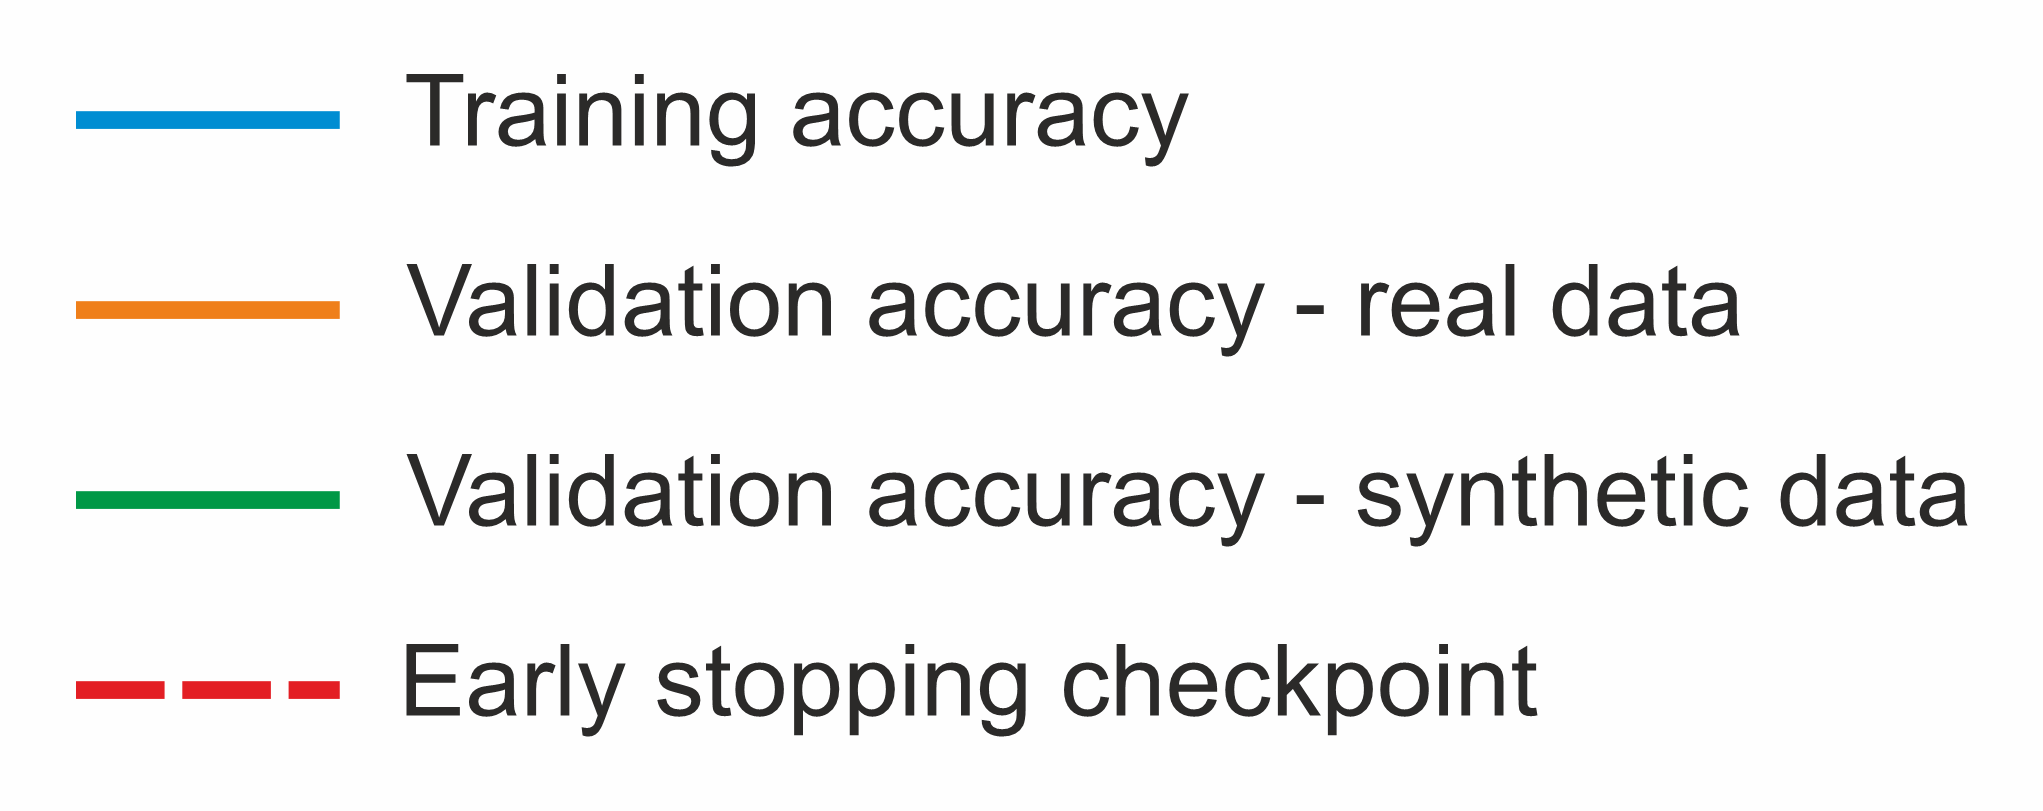
\includegraphics[width=.7\textwidth]{images/popisAc.png}
        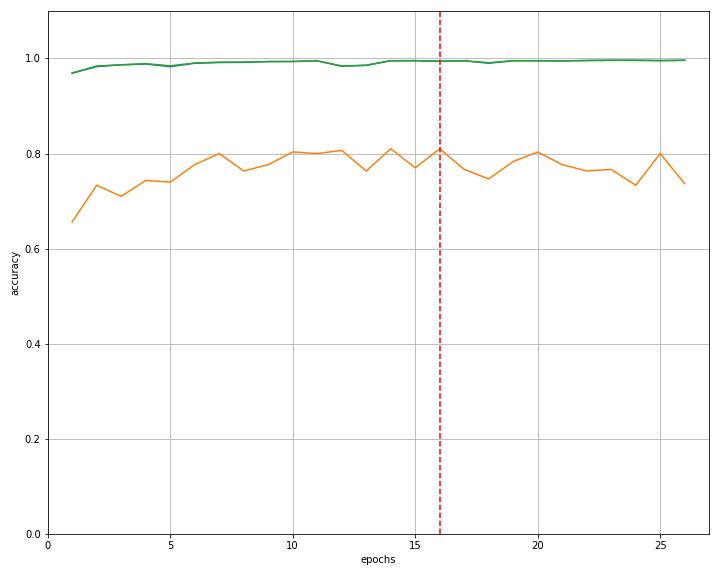
\includegraphics[width=\textwidth]{images/accuracy51ss2_0.png}
        \caption{The accuracy during training.}
        \label{fig:accm22}
    \end{subfigure}
    \begin{subfigure}[t]{.45\textwidth}
        \centering
        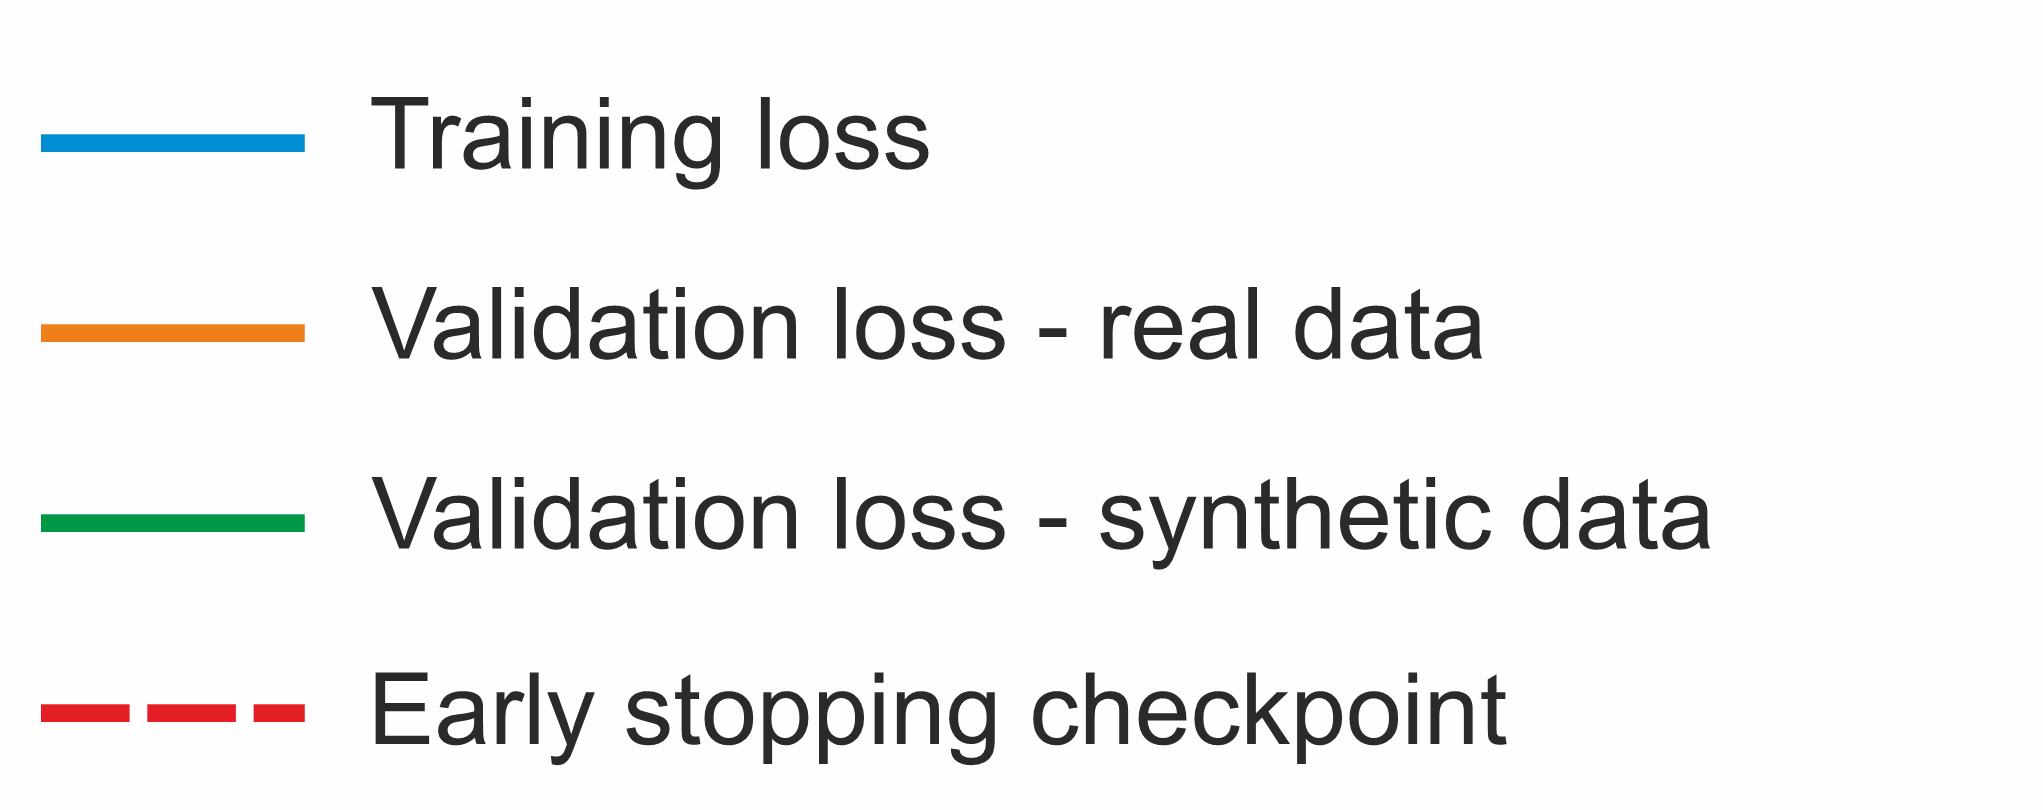
\includegraphics[width=.7\textwidth]{images/popisLoss.png}
        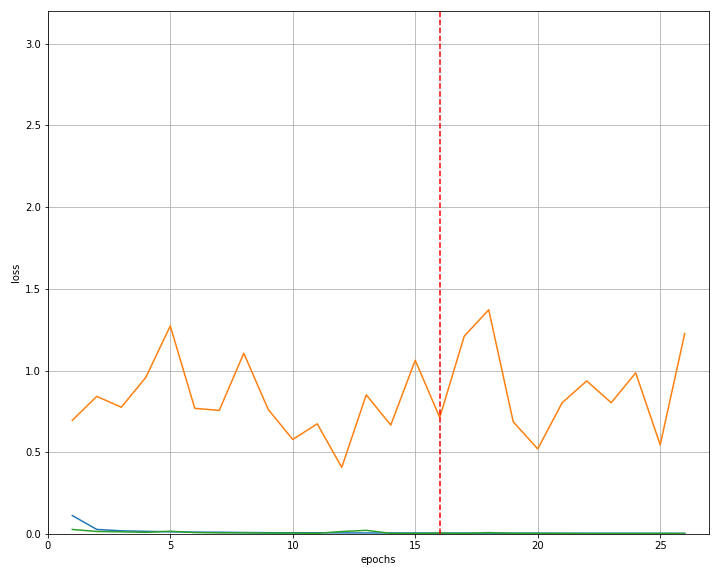
\includegraphics[width=\textwidth]{images/losses51ss2_0.png}
        \caption{The loss during training.}
        \label{fig:lossm22}
    \end{subfigure}

    \caption{The evolution of the loss and accuracy during training of the final model on the synthetic data.}
    \label{fig:lossaccm22}
\end{figure}








